
\documentclass[12pt,english]{article}
\usepackage{mathptmx}

\usepackage{color}
\usepackage[dvipsnames]{xcolor}
\definecolor{darkblue}{RGB}{0.,0.,139.}

\usepackage[top=1in, bottom=1in, left=1in, right=1in]{geometry}

\usepackage{amsmath}
\usepackage{amstext}
\usepackage{amssymb}
\usepackage{setspace}
\usepackage{lipsum}

\usepackage[authoryear]{natbib}
\usepackage{url}
\usepackage{booktabs}
\usepackage[flushleft]{threeparttable}
\usepackage{graphicx}
\usepackage[english]{babel}
\usepackage{pdflscape}
\usepackage[unicode=true,pdfusetitle,
 bookmarks=true,bookmarksnumbered=false,bookmarksopen=false,
 breaklinks=true,pdfborder={0 0 0},backref=false,
 colorlinks,citecolor=black,filecolor=black,
 linkcolor=black,urlcolor=black]
 {hyperref}
\usepackage[all]{hypcap} % Links point to top of image, builds on hyperref
\usepackage{breakurl}    % Allows urls to wrap, including hyperref

\linespread{2}

\begin{document}

\begin{singlespace}
\title{Classifying Beer by Alcoholic Volume\thanks{Data used with permission from Kaggle}}
\end{singlespace}

\author{Michael Yuhas\thanks{Department of Economics, University of Oklahoma.\
E-mail~address:~\href{mailto:MYuhas5120@ou.edu}{MYuhas5120@ou.edu}}}

% \date{\today}
\date{May 8, 2018}

\maketitle

\begin{abstract}
\begin{singlespace}
Using data from over two thousand four hundred craft beers, machine learning algorithms for K Nearest Neighbors and Support Vector Machines are employed in an effort to predict beer type given its alcoholic content by volume.  Predictive algorithms similar to this can be used to find new market niches for breweries to fill.
\end{singlespace}

\end{abstract}
\vfill{}


\pagebreak{}


\section{Introduction}\label{sec:intro}
Over the past ten years, the United States(U.S.) market for liquor has been slowly growing.  Beer sales have lost some of their share of the U.S. liquor market in the past five years, decreasing by 1.6\% in 2017 alone; however, craft beer has increased its share of the beer market overall, increasing its share by 5.0\%  in 2017\citep{BrewersFriend2}.  Craft breweries advertise based on their traditional brewing techniques and small batch size.  This focus on small-scale production leads to a greatly diverse product set with a heavy emphasis on marketing and consumer taste preferences, an excellent example of a monopolistic market.

Due to the the increased competition from additional producers entering the market, craft breweries are under consistent pressure to maintain what share of the consumers they can through brand quality and loyalty.  Additionally, they must constantly strive to offset the effects of consumer base erosion by attempting to find new ways to entice potential customers, both those new to the market and those from other brewery consumer bases.  There are two primary ways of attracting new consumers.  Traditionally, the less costly of the two methods is more marketing, either the same marketing in a new area or a new campaign for an existing area of target.  The other alternative is to find a new sub-market to create a product for, something that will appeal to consumers by giving them a new taste to prefer.  Do to the relatively small size of craft breweries and their emphasis on small-scale production the latter option for consumer attraction is less costly than for other markets, that for soda for instance.

Another common point of interest in the craft beer market is alcoholic content as measured by Alcohol by Volume(ABV).  There are market niches on both ends of the spectrum, either selling beers with much higher than average ABV's or much lower.  By creating predictive algorithms that can use alcoholic content of a craft beer to help ascertain the style of the beer, the hope is to provide pieces of the puzzle of what exactly consumers prefer in a drink in order to help progress market research into what types of brews to create next.  

\section{Literature Review}\label{sec:litreview}
work done by \citet{elzinga_tremblay_tremblay_2015} has taken on the task of tracking the history of the craft beer industry starting in the nineteen seventies and continuing on to the present day.  They have also compiled a database of statistical information and analysis using metrics that would effect the rise of the industry.  They found that between 1976, when the first craft brewery opened, and 2015 when the study was taken craft beer production had risen from four hundred barrels annually to close to 13.2 million barrels annually.  Furthermore, the number of breweries has been growing almost continuously since 1980 with the exceptions of periods between 1997-99 and 2003-2004, finishing with the presence of 2500 craft breweries in 2013.  By 2017 productions levels for craft beer had reached 17.9 million barrels\citep{BrewersFriend}, a 4.7 million barrel increase in just two years which indicates that growth is still occurring at an accelerated pace with no signs of slowing.

The craft beer industry has had a visible effect on the greater economy as a whole too according to \citet{thompson_2018} in The Atlantic.  According to him via the Bureau of Labor Statistics, total employment at U.S. breweries has increased by over 300\% between 2001 and 2017, reaching nearly seventy thousand jobs by the middle of 2017.  According to market economists interviewed for the article, one of the prevailing causes for the increase in the craft beer industry is consumer preferences.  Craft breweries have started to fill the niche taste markets that industry giants have ignored.  This is also contributing to economic growth for the regions they start in providing jobs and new products decentralized from the breweries of much larger producers.  

The importance of taste preferences is emphasized further by research done by \citeauthor{beersnobs}.  In their article, Beer Snobs Do Exist: Estimation of Beer Demand by Type, they analyze data on beer type and pricing in order to determine market overlap between different types of producers.  They also determined that styles of beer were often of significance in terms of market share.  There research concluded that there were essentially totally different markets for beer based on type, i.e. craft, import, or mass produced, using cross-price elasticity analysis.  They also hypothesized that craft beers share of the overall market would continue to grow as it had for their entire period of study.  Their statistical confirmation of the importance of taste preferences in the market provides significance to the search for finding new preference sets to create products for.

Brewers Friend, an organization that provides educational services for craft brewing compiled a chart indicating the existing range of ABV's for different styles of craft brew \citep{BrewersFriend}.  This indicates current possible preference sets for which there are already products available.  In the future this data may be used to help identify missing preference sets using predictive models based on current consumption patterns of various taste attributes.

\section{Data}\label{sec:data}
Data for this research came from a data-set published on Kaggle \href{https://www.kaggle.com/nickhould/craft-cans/data}{here}. Table \ref{tab:descriptives} contains summary statistics.

The original data set contains data on two thousand four hundred and ten beers with values for ABV, ibu(International Bittering Unit), beer name, beer style, brewery, and quantity in ounces.  Due to numerous missing values for ibu, the variable was not chosen for research.  Due to a lack of requisite knowledge of text analysis and inherent uniqueness beer name was also disqualified.  Brewery data was complete for most data values but had some problematic overlapping missing values where entire breweries had missing data values for other variables and was therefore disqualified until such time as missing values can be found and added.

ABV is a continuous variable with range between 0.01 and 0.128 representing the percentage of alcohol by volume in a beer.  Ounces is also a continuous variable and represents the quantity of the beverage per container; this ranges from 8.4 to 32 ounces.  There is a moderate likelihood of collinearity between ABV and ounces as beers with a higher ABV are sometimes served in a smaller quantity than other beers.  However, due to focus on out of sample predictive capability, they shall both be included in the algorithsm.  Style is a categorical variable containing one hundred different possible outcomes.

After removing data points where ABV values, ounces, or style types were missing, the data set contained 2348 observations.  80\% of the data was randomly selected to be included in the training set and the remainder was placed into the testing set.  One problem that came up was the training set containing different styles than were also present in the testing set.  In order to complete the modeling with truly randomized data, the algorithm task was instructed to not try to fix or find any inconsistencies.  Another alternative would have been to set up stratified sampling for the entire data set in order to ensure the same potential style outcomes for training and testing, but due to the non-negligible number(17) of styles containing 2 or fewer data points and the preference for truly random sampling this was not done.  


\section{Empirical Methods}\label{sec:methods}
My analysis employed both K nearest neighbors and support vector modeling due to their similar nature; however the basic empirical model is the same for both and can be seen in the following equation:

\begin{equation}
\label{eq:1}
Y_{ij}=\alpha_{0} + \alpha_{1}Z_{ij} + \alpha_{2} X_{ij} + \varepsilon,
\end{equation}
where $Y_{ij}$ is a categorical outcome variable for ABV value $i$ by ounces $j$, and $Z$ are the range of possible ABV values known for this style $Y$, while $X$ are known possible ounce values of style $Y$. The parameter of interest is $Y_{ij}$ after finding optimal values for $\alpha_{1}$ and $\alpha_{2}$.

More specifically, the parameter of interest is the predictive accuracy of $Y_{ij}$ given ABV and ounces. Using K nearest neighbors, the algorithm searches for similar values of the two variables and their style and uses that to predict the style of the current data set.  

Support vector modeling works similarly.  A three dimensional space is created with each axis representing a different variable and hyper planes are drawn between known data points at a maximum distance from the nearest data point in any given category of style.  Using these hyper-planes as cutoff points, the support vector machine predicts any new data point's style type given its values for ABV and ounces.

In order to find maximize the accuracy, the models are first tuned using ten different random samples drawn from the training data that was set aside from the overall data set.  The tuning process finds the optimal values for $\alpha_{1}$ and $\alpha_{2}$ given the training data used.  Once these values are found, the algorithm is told to use these to make predictions.  The algorithm's performance is then retested in order to verify the strength of the parameters.  Once this is done, the final algorithm is set with the optimal parameters and then used to create predictions using the data in the test data set.  The performance of these predictions is then tested for accuracy and the average accuracy for all predictions is reported as a measure of the algorithms strength.


\section{Research Findings}\label{sec:results}
The K nearest neighbors algorithm had a predictive accuracy value of 0.2638 or 26.38\%.  The support vector model algorithm had a predictive accuracy value of 0.2808 or 28.08\%.  While the support vector model had a definite lead in predictive accuracy, the capability of both algorithms is still greatly lacking.

The optimal parameter settled on for the K nearest neighbors algorithm was 39 neighbors with possible values between one and forty which may indicate that more neighbors may be added without overfitting the algorithm to the given data.

The support vector model's improved performance comparatively is most likely attributable to it being better suited to multiple classification.  Since it relies less on physical data points and more on the space surrounding them in a theoretical hyper-plane, the geometric calculations have the capability of being more accurate and creating better boundary points between predictions for different beer styles.

Despite the low predictive power of the algorithms, having a one in four chance of predicting a beer's style out of the one hundred style's possible indicates some level of useful correlation between style and ABV and ounces.  


\section{Conclusion}\label{sec:conclusion}
The low predictive power of both algorithms signals that ABV and ounces are not sufficient information to consistently predict the style of beer.  One option would be to condense the options for style into four or five main branches; however, this would do nothing to help the long-term goal of product research for new market niches to expand into.  Furthermore, given craft beers heavy emphasis on small scale production of a greater variety of tastes it would also be a counter-intuitive move.

A more preferable option is to add in other variables that would logically add to the predictive power.  The first to be added should be brewery identification data as it will be a simple if tedious process to obtain the information required to fill in the missing not at random gaps in the data.  The next step to improving predictive power of the algorithms would be to add in beer name as another variable.  It will be more difficult to properly use this data as string identification should be applied to both the beer names and the styles in order to find key matching words that will narrow the selection process.  For instance, many styles of pale ales incorporate the word pale or ale into their names which would help narrow the likely list of styles from one hundred down to fifteen or so.  Another variable to potentially add would be ibu, international bittering unit; however, the amount of missing data points is significant and more research would be required to ensure that ibu is available for all craft brews.

Considering the relative predictability of the models compared to a draw at random chance, 25\% is a significant improvement to 1\%.  This indicates a use-able correlation between ABV and ounces and beer style.  In addition to using the above suggestions to increase the predictive strength of the algorithms, it may be useful to try other types of algorithms that are better suited to working with greater numbers of variables.

Looking onward, as the predictability of the model is improved with added variables, pricing, cost, and profit analysis should also be done on beer styles to determine which niches would be the easiest to move into and which will have the greatest profitability.  This analysis should be also be done with data collected for other studies, some mentioned earlier, in order to find regions of greatest possibility for market growth as well as trying to determine ABV/style combinations that are most desired by consumers.

\vfill
\pagebreak{}
\begin{spacing}{1.0}
\bibliographystyle{jpe}
\bibliography{Citations.bib}
\addcontentsline{toc}{section}{References}

\end{spacing}

\vfill
\pagebreak{}
\clearpage

%========================================
% FIGURES AND TABLES 
%========================================
\section*{Figures and Tables}\label{sec:figTables}
\addcontentsline{toc}{section}{Figures and Tables}
%----------------------------------------
% Figure 1
%----------------------------------------
\begin{figure}[ht]
\centering
\bigskip{}
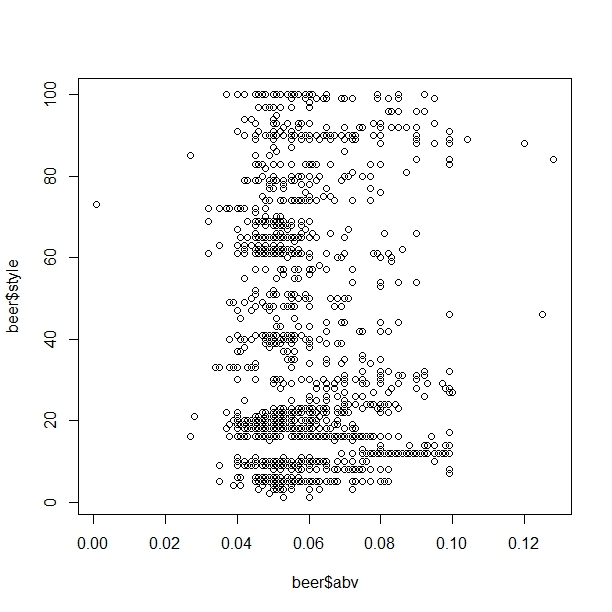
\includegraphics[width=.9\linewidth]{Plot.jpeg}
\caption{Range of ABV for each beer style}
\label{fig:fig1}
\end{figure}

%----------------------------------------
% Table 1
%----------------------------------------

% Table created by stargazer v.5.2 by Marek Hlavac, Harvard University. E-mail: hlavac at fas.harvard.edu
% Date and time: Tue, May 07, 2018 - 5:42:18 PM
\begin{table}[!htbp] \centering 
  \caption{Summary Statistics of Variables of Interest} 
  \label{tab:descriptives} 
\begin{tabular}{@{\extracolsep{5pt}}lccccc} 
\\[-1.8ex]\hline 
\hline \\[-1.8ex] 
Statistic & \multicolumn{1}{c}{N} & \multicolumn{1}{c}{Mean} & \multicolumn{1}{c}{St. Dev.} & \multicolumn{1}{c}{Min} & \multicolumn{1}{c}{Max} \\ 
\hline \\[-1.8ex] 
abv & 2,348 & 0.060 & 0.014 & 0.001 & 0.128 \\ 
ounces & 2,348 & 13.592 & 2.333 & 8.400 & 32.000 \\ 
\hline \\[-1.8ex] 
\end{tabular} 
\end{table} 


\end{document}
